\documentclass[answer]{cphos}

\cphostitle{CPHOS物理竞赛联考}
\cphossubtitle{理论试题命题模板}

\setscorecheck{true} 

\begin{document}
\begin{problem}[40]{啊啊啊宝宝你是一个软软的小蛋糕} 

\begin{problemstatement}
笔者于某次集训的酒店吃早饭时观察到，如果使用筷子击打一小块蛋糕的底部，蛋糕会滑动并在一个新的位置停下，然后开始很可爱的摇头晃脑。本题将以一个有趣但未必正确的方式来解释这一现象。

\subq{1} 
首先可以想到的是，我们可以把蛋糕简化为一根长宽高分别为$a,b,l$的匀质刚体（$a$ 为垂直纸面的宽度），其质量为$m$，且$a,b\ll l$。如下图黑线所示，其底端被铰链固定，宽垂直于纸面方向。将其从$\theta=0$处静止释放，其会向下旋转，重力加速度为$g$。求出这一过程中的$\dot{\theta}$和$\ddot{\theta}$，本问不考虑 $a,b$ 的影响。

\begin{figure}[H]
	\centering
	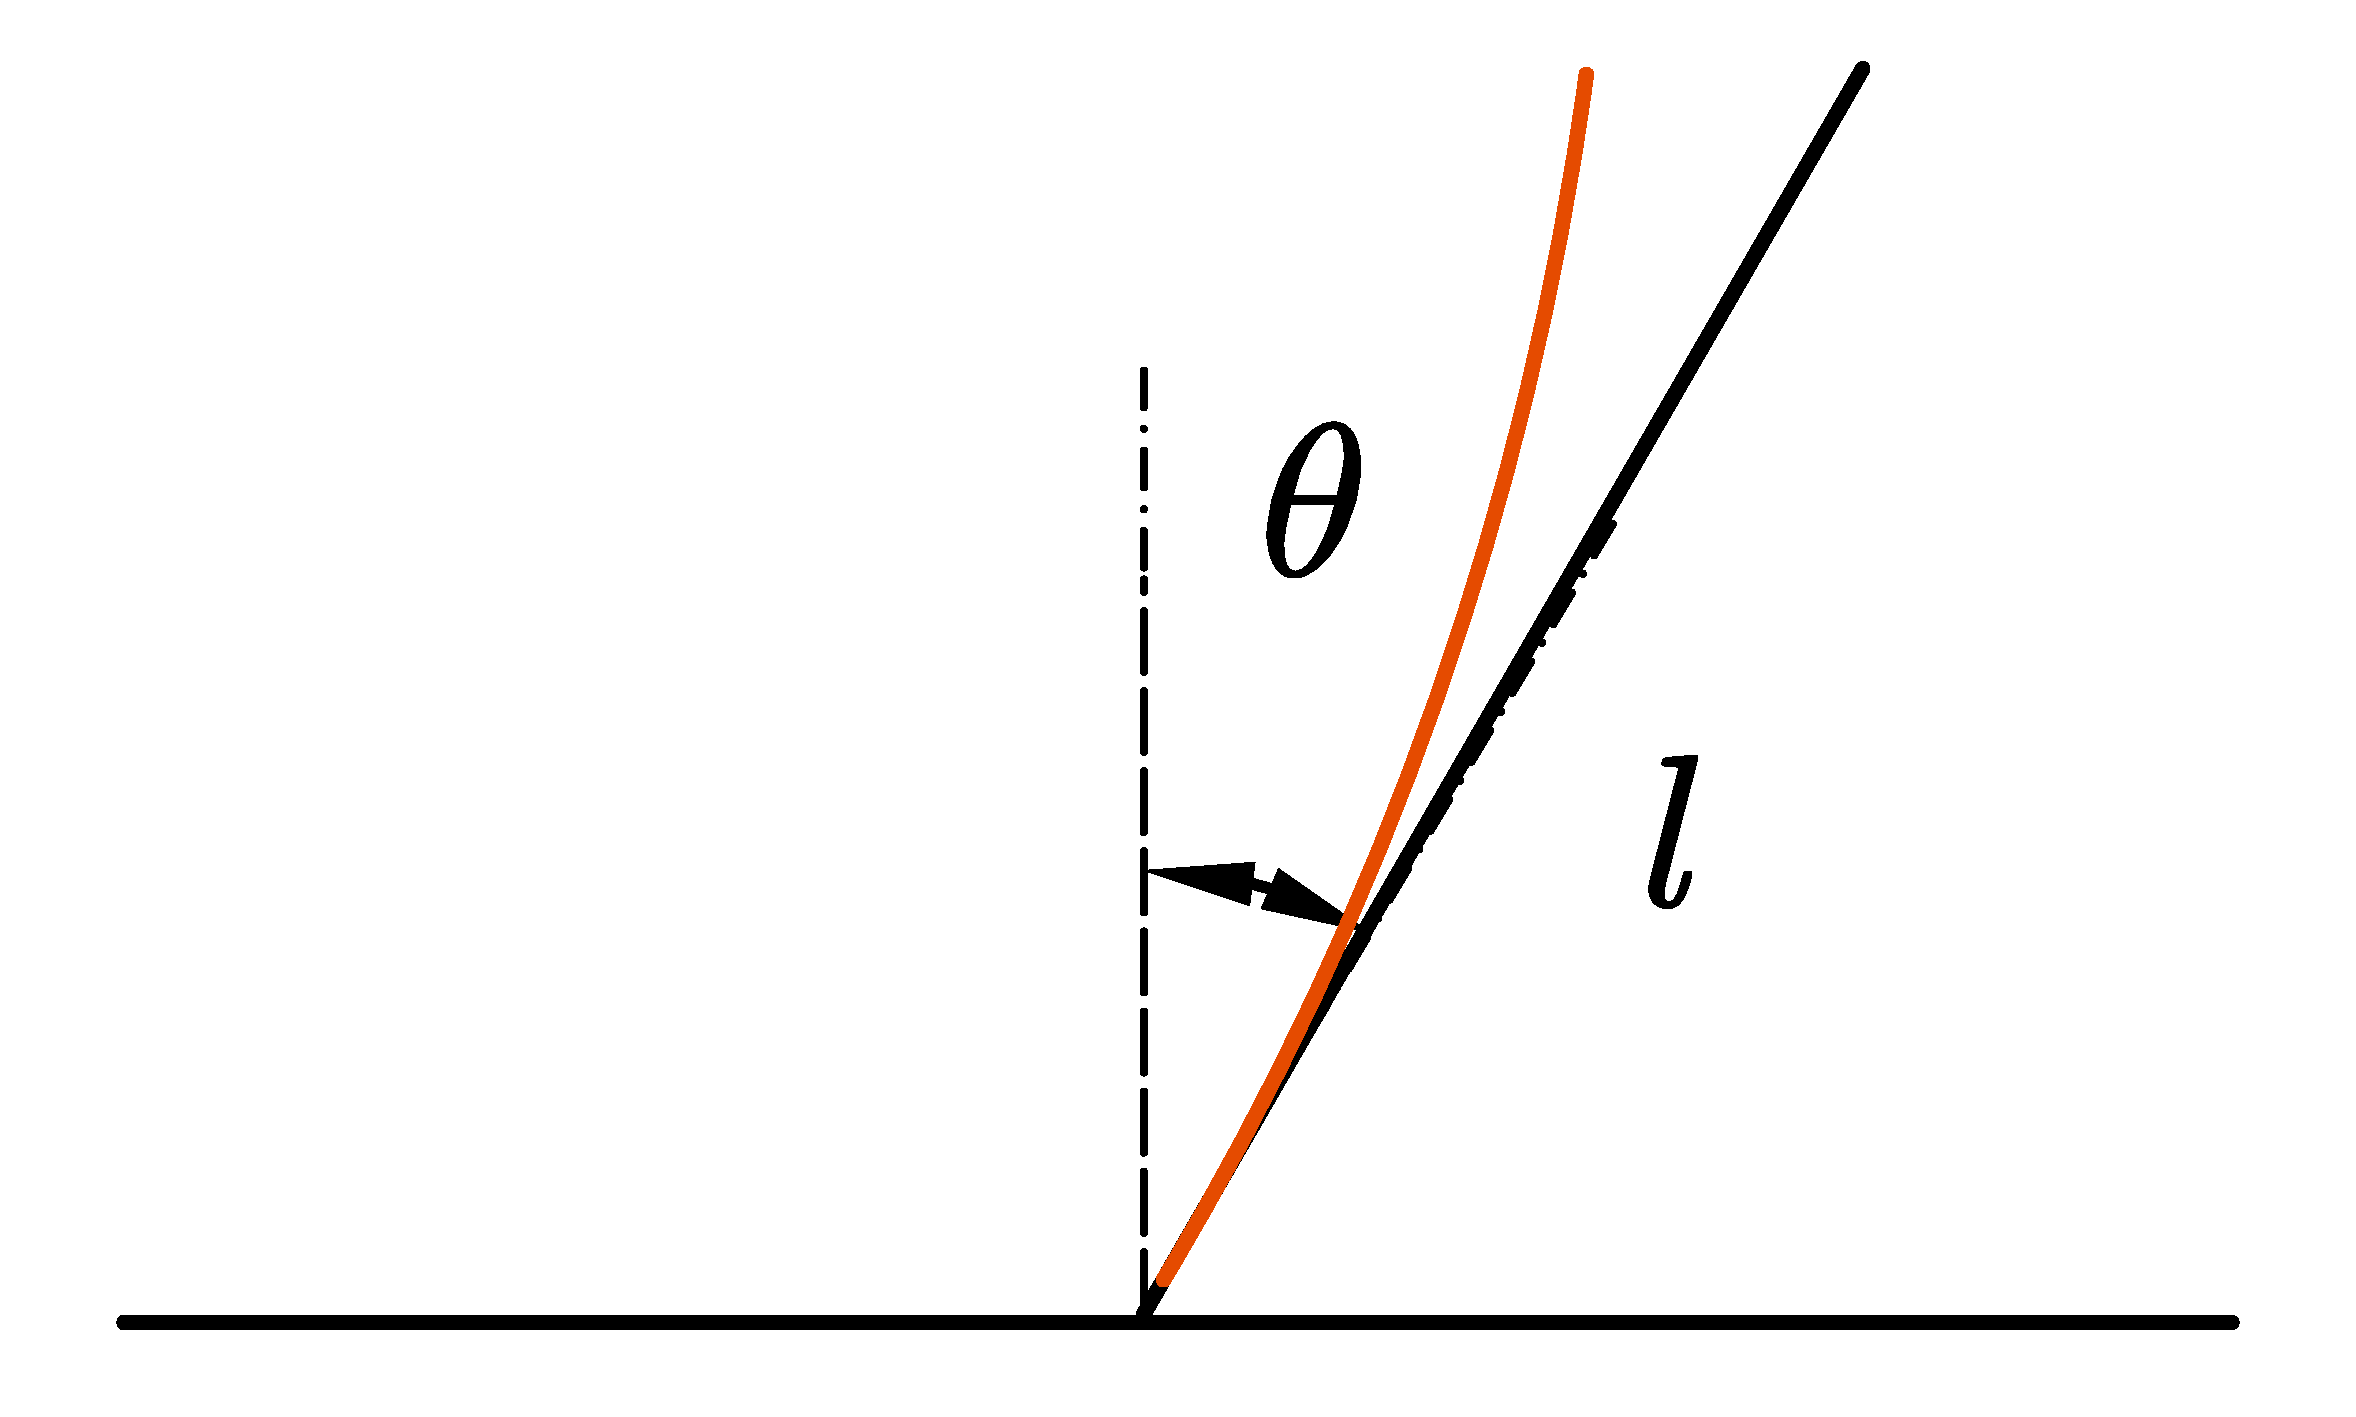
\includegraphics[width=0.4\textwidth]{assets/1p2_1.pdf}
	\caption{蛋糕模型简化示意图}
	\label{fig:1p2_1}
\end{figure}

\subq{2}
求出为了使整个刚体同步转动，其距底端$xl$处的切向应力$F$和应力矩$M$。


\subq{3}
想必你一定注意到了上图中的红线。因为其有杨氏模量$E$，在上问的力矩$M$下，其会发生形变，如红线所示。假设形变较小，求出距底端$xl$处实际形状较原形状的偏离$y$。

\subq{4}
由于形变，其受到的总重力矩发生了$\Delta M$的变化。在最低阶近似下求出该变化。

\subq{5}
在上述的简化情况下，求出在$\theta=0$附近振动的角频率$\omega$。这需要$E$满足什么条件？譬如，取蛋糕为$1\text{~cm}\times 1\text{~cm}\times 3\text{~cm}$，密度$1000\text{~kg/m}^3$，估算临界杨氏模量$E_c$的数值。

\subq{6}
讨论该模型有哪些问题。

\end{problemstatement}

\begin{solution}

\solsubq{1}{3}
根据能量守恒 $\dfrac12mgl(1-\cos\theta)=\dfrac16ml^2\dot\theta^2$，结合 $\ddot\theta=\dfrac{\mathrm{d}\dot\theta^2}{2\,\mathrm{d}\theta}$ 得到：
\begin{equation}
	\dot{\theta}=\sqrt{\frac{3g(1-\cos\theta)}{l}},\quad \ddot{\theta}=\frac{3g\sin\theta}{2l} \eqtagscore{1}{3}
\end{equation}

\solsubq{2}{6}
对最上方 $l-xl$ 段分析受力，有

\begin{equation}
	\begin{aligned}
		F&=(1-x)m(g\sin\theta-r\ddot\theta)=(1-x)m\left(g\sin\theta-\frac{1+x}{2}l\cdot\frac{3g\sin\theta}{2l}\right) \\
		&=\frac{mg\sin\theta}{4}(1-3x)(1-x)
	\end{aligned} \eqtagscore{2}{3}
\end{equation}

\begin{equation}
	M=\int_0^{xl}F\,\mathrm{d}x\cdot l=\frac{mgl\sin\theta}{4}x(1-x)^2 \eqtagscore{3}{3}
\end{equation}

\solsubq{3}{9}
截面抗弯矩

\begin{equation}
	E_0=E\iint z^2\,\mathrm{d}S=Ea\int_{-b/2}^{b/2}z^2\,\mathrm{d}z=\frac{Eab^3}{12} \eqtagscore{4}{3}
\end{equation}

又因为

\begin{equation}
	y''=\frac{M}{E_0} \eqtagscore{5}{2}
\end{equation}

代入积分得

\begin{equation}
	y=\frac{3mgl^3\sin\theta}{Eab^3}\left(\frac{x^5}{20}-\frac{x^4}{6}+\frac{x^3}{6}\right) \eqtagscore{6}{4}
\end{equation}

\solsubq{4}{6}
附加力矩

\begin{equation}
	\Delta M=\int_0^1-mgy\cos\theta \,\mathrm{d}x=-\frac{m^2g^2l^3\sin\theta\cos\theta}{20Eab^3} \eqtagscore{7}{6}
\end{equation}

\solsubq{5}{12}
总力矩

\begin{equation}
 M_t=\left(\frac{mgl}{2}-\frac{m^2g^2l^3}{20Eab^3}\right)\sin\theta\eqtagscore{8}{2}
\end{equation}

\begin{equation}
	I=\frac{ml^2}{3}\eqtagscore{9}{1}
\end{equation}

根据 $M_t=I\ddot\theta$ 并作小量近似，有

\begin{equation}
	\frac{mgl}{2}-\frac{m^2g^2l^3}{20Eab^3}+\frac{ml^2}{3}\omega^2=0 \eqtag{10}
\end{equation}
\begin{equation}
	\omega=\sqrt{\frac{3mg^2l}{20Eab^3}-\frac{3g}{2l}} \eqtagscore{11}{3}
\end{equation}

要求

\begin{equation}
	E<\frac{mgl^2}{10ab^3}\eqtagscore{12}{2}
\end{equation}

譬如，取蛋糕为$1 \text{~cm}\times1 \text{~cm}\times3 \text{~cm}$，密度$1000 \text{~kg/m}^3$，估算可得$E=270 \text{~Pa}$。\addtext{结果与 $270 \text{~Pa}$ 差一个数量级以内均可得}{4}

\solsubq{6}{4}

1.算出的杨氏模量太小，显然不合理；

2.忽略了内部质点的上下振动；

3.计算出的附加力矩会反作用于运动，从而再反过来使力矩变化；

4.水平线度并不远小于竖直线度；

等等。\addtext{言之有理即可；答出一个方面2分，两个方面及以上}{4}

\scoring
\end{solution}

\end{problem}

\end{document}
